%\chapter{Symbole przyjęte w pracy}
%\label{app:symbole}

%Jeśli w tekście nie wykazano inaczej, stosowane symbole należy rozumieć jako:

%\begin{itemize}
%\item[$f(x,y)$] - jasność piksela o współrzędnych $(x,y)$ w obrazie wejściowym,
%\item[$g(x,y)$] - jasność piksela o współrzędnych $(x,y)$ w obrazie wynikowym,
%\item[$t$, $t_i$] - wartości progowe,
%\item[$G$] - liczba poziomów szarości obrazu; $G=256$,
%\item[$P(i,j)$] - macierz GLCM,
%\item[$M(i,j)$] - maska przetwarzania.
%\end{itemize}


%%%%%%%%%%%%%%%%%%%%%%%%%%%%%%%%%%%%%%%%%%%%%%%%%%%%%%%%
\chapter{AchillesDL: System komputerowego wspomagania oceny gojenia ścięgien i więzadeł}
\label{app:AchillesDL}
\begin{figure}[H]
	\centering
	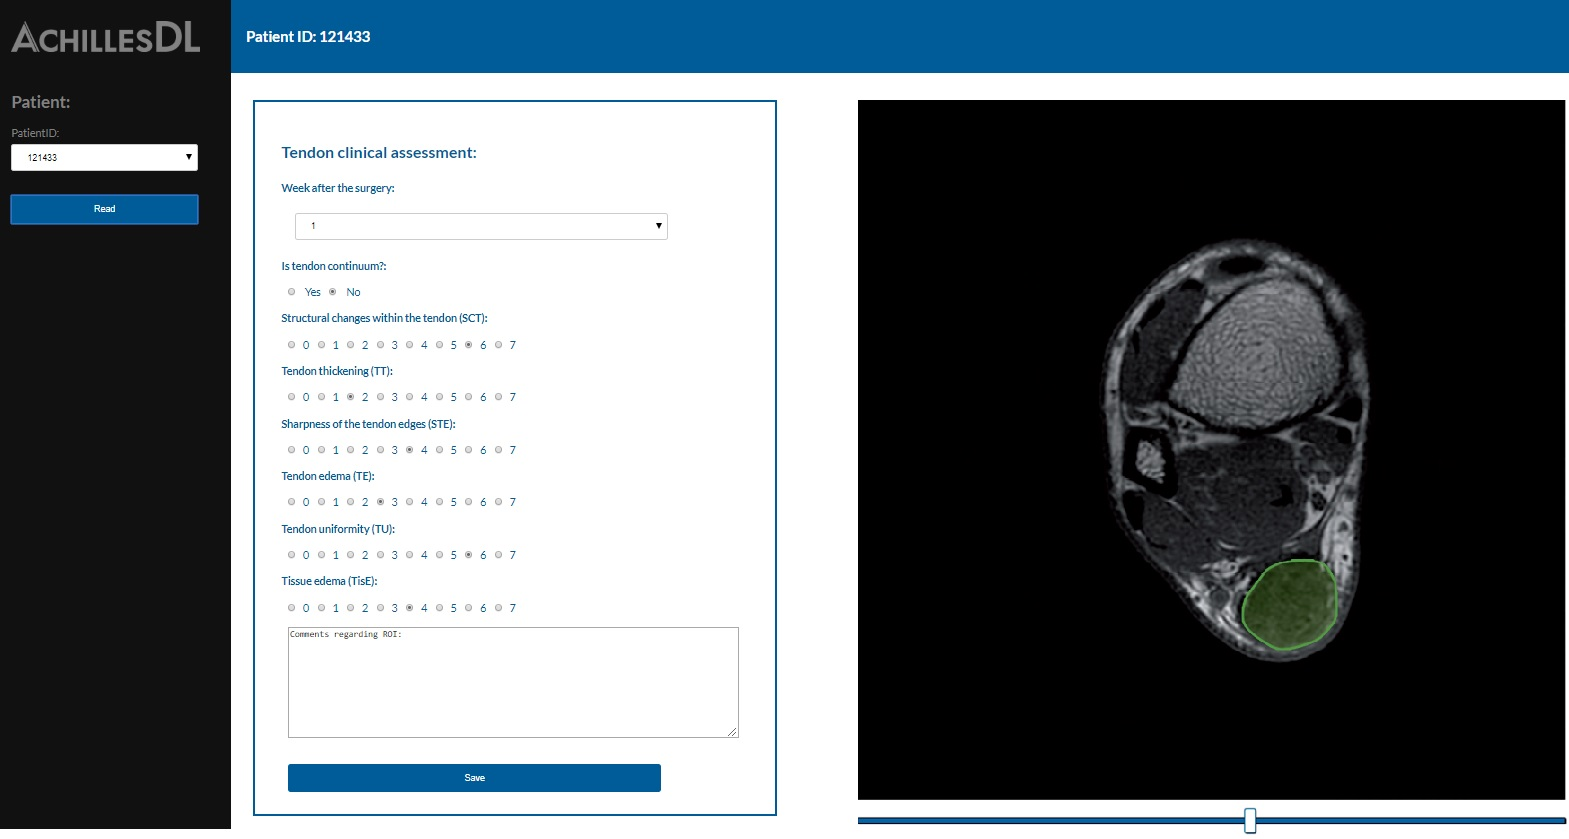
\includegraphics[width=1\textwidth]{figures/achillesDL.jpg}
	\caption{Front-end aplikacji AchillesDL przeznaczonej do oznaczania badań RM ścięgna Achillesa.}\label{fig:achillesDL}
\end{figure}
W ramach projektu START powstał rozwijany przez autora tej pracy system AchillesDL służący do intuicyjnego przeglądania i etykietowania danych radiologicznych z wykorzystaniem przeglądarki internetowej. System ten został zaprezentowany na konferencji NVIDIA GTC 2018 w San Jose, Kalifornia \cite{KapinskiGTC2018}. Front-end aplikacji można zobaczyć na Rys. \ref{fig:achillesDL}.


System umożliwia:
\begin{itemize}
	\item wybór pacjenta z menu rozwijanego widocznego po lewej stronie ekranu;
	\item wizualizację badań RM w różnych przekrojach;
	\item wypełnienie i zapis ankiety omówionej w p. \ref{seq:ground-truth}.
\end{itemize}

Trwają również prace nad wizualizacją wyników oceny automatycznej wraz ze wskazaniem w 2D i 3D obszarów zainteresowania sieci. Po wcześniejszym skontaktowaniu się z autorem tej pracy pod adresem mailowym norkap@icm.edu.pl możliwy jest dostęp do systemu poprzez stronę achillesdl.icm.edu.pl.